\section{Theoretic Foundations}
\label{sec:Theorie}

\subsection{The LHCb detector}

The LHCb experiment is one of the four larg experiments located at the Large Hadrom Collider (LHC) at CERN. 
This analysis is concerned with data from proton collisions from run 2 (2015-2018) of the experiment where proton bunches were collided at 
a center of mass energy of $13 \, \si{\tera\eV}$ with a frequency of $40 \cdot 10^6 \, \si{\hertz}$. The LHCb experiment studies mainly hadrons 
containing a charm or a bottom quark. It allows precision measurments of flavor physics processes. 
The composition of the LHCb detector is shown in figure \ref{f1}. \\
The Vertex Locator (VELO) is a silicon strip detector measuring tracks of charged particles and therefore enabling the location of the 
primary vertex (PV) and secondary vertices of particles that decay in the VELO. The tracking stations TT, T1, T2 and T3 consist of four-layer silicon 
strip detectors and drift tubes and allow the reconstruction of tracks of charged particles and, in combination with the magnet, the reconstruction of the 
particles momenta.
The Ring Imaging Cherenkov Detectors (RICH) RICH1 and RICH2 allow for the roconstruction of the particles velocity via cherenkov radiation. 
Cherenkov radiation is emitted if a charged particle is traveling faster than the speed of light in a material with an opening angle determined by 
\begin{equation}
  \cos (\theta) = \frac{1}{n \beta}
\end{equation}
where $n$ is the refractive index of the material. 
Combining information on a particles velocity and momentum allows for the reconstruction of a particles mass. 
%Furthermore the condition posed 
%by the speed of light in the detector material is used to distinguish protons, kaons and pions from each other due to the use of different materials.  
The calorimeter system consists of the Scintillation Pad Detector (SPD), the Pre Shower detector (PS), and the electromagnetic calorimeter (ECAL) 
as well as the hadronic calorimeter (HCAL). The ECAL and HCAL both are sampling calorimeters with absorber layers of either iron or lead. 
The system allows for the identification of photons, electrons and hadrons and the measurement of the particles energies. The photons and electrons 
deposit their energy mainly in the ECAL while hadron deposit most of their energy in the HCAL.
%The electromagnetic calorimeter (ECAL) allows for the measurement of the energy of photons and electrons while the hadronic calorimeter (HCAL)
%allows for the measurement of the energy of hadrons.
The muon system M1 to M5, consisting of alternating iron absorbtion layers and multy wire chambers, allows for the identification of muons which are 
the only particles after the calorimeter system since they are minimally ionizing particles.

\begin{figure}[!htb]
    \centering
    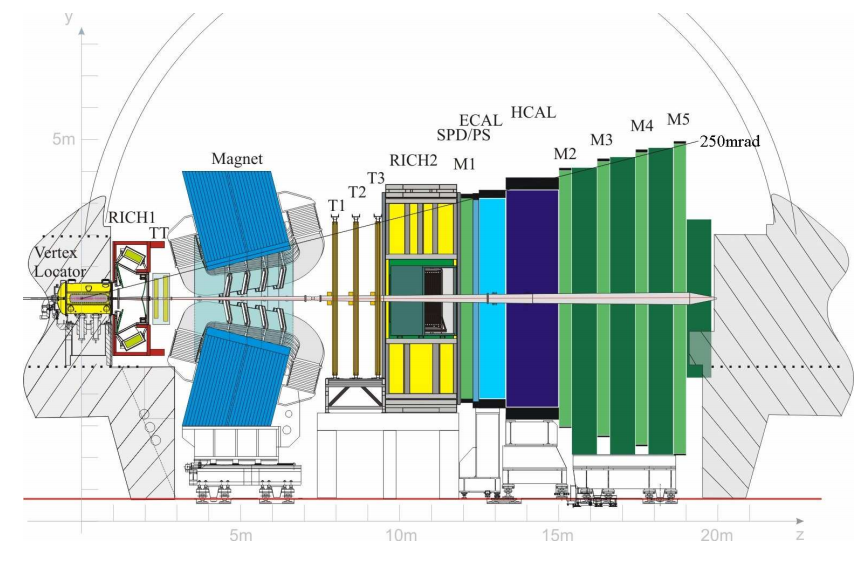
\includegraphics[width=0.8\textwidth]{graphics/lhcb.png}
    \caption{Components of the LHCb detector. \cite{sample_cpv}}
    \label{f1}
  \end{figure}



\subsection{The $B_s^0$ decay}
The studied decay in this analysis is the flavor changing weak decay $B_s^0 \rightarrow \psi(2S) K_s^0$.
A leading order feynman diagram for the decay is shown in figure \ref{f2}. 
Since the final state particles of the decay are not measured directly secondary decays of the $\psi(2S)$ and $K_s^0$ 
have to be considered for the analysis. 
%utilized in the analysis are discussed. \\
%, from which the decay 
%of the $B_s^0$ is reconstructed in the analysis 
%Since the decay products are not measured directly the secondary decays have to be discussed. \\
The $\psi(2S)$ decays mainly via the strong interaction due to its valence quark content of $c \overline{c}$. 
%The quark content of $\psi(2S)$ is $c \overline{c}$ and it decays dominantly via the strong interaction. 
To reduce errors due to misidentification of final state 
particles the decay $\psi(2S) \rightarrow \mu^+ \mu^-$ with a branching fraction of $\mathcal{B}(\psi(2S) \rightarrow \mu^+ \mu^-) 
(8.0 \pm 0.6) \cdot 10^{-3}$ \cite{pdg} is used in the analysis. To exclude other particles containing $c\overline{c}$ 
the invariant mass of the muons is restricted to $m(\mu^+ \mu^- ) \approx m(\psi(2S))$ .\\ 
The $K_s^0$ decays dominaltly via a weak decay to $\pi^+ \pi^-$. This decay, which is used in the analysis, has a braching fraction of 
$\mathcal{B}(K_s^0 \rightarrow \pi^+ \pi^-) = (69.20 \pm 0.05) \, \%$ \cite{pdg}. \\
%The $K_s^0$ has as quark content a superposition of $d \overline{s}$ and $\overline{d}s$. The dominant decay mode, which will be used in the analysis, 
%is $K_s^0 \rightarrow \pi^+ \pi^-$ with a branching fraction of $\mathcal{B}(K_s^0 \rightarrow \pi^+ \pi^-) = (69.20 \pm 0.05) \, \%$ \cite{pdg}. \\
The data contains a significant number of background events from combinatorial background and the decay $B^0 \rightarrow \psi(2S) K_s^0$. 
The decay $B^0 \rightarrow \psi(2S) K_s^0$ is kinematically similar to the studied decay and passes all the selection criteria discussed so far. 
The invariant mass of the $B^0$ events shows a sharp peak that is smeared out due to the detector resolution. 
Combinatorial background results from wrongly combined events that do not originate from the decay of the $B^0$. The invariant mass of the 
combinatorial background is distributet randomly. 
To separate the signal from the decay $B_s^0 \rightarrow \psi(2S) K_s^0$ from the various backgrounds a Boosted Decion Tree (BDT) is implemented. 

  \begin{figure}[!htb]
    \centering
    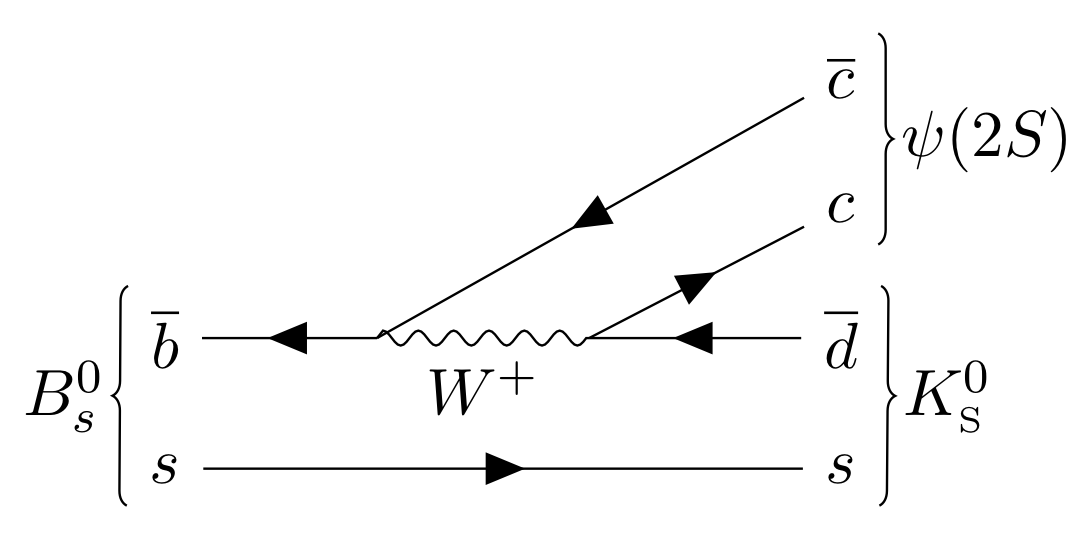
\includegraphics[width=0.4\textwidth]{graphics/image.png}
    \caption{A leading order feynman diagram for the decay $B_s^0 \rightarrow \psi(2S) K_s^0$. \cite{sample}}
    \label{f2}
  \end{figure}